\chapter{Phase  Plane Diagrams: COMING SOON}
\label{ch-phase-plane}

This chapter is based on Ref.\cite{wiki-phase-plane}.


\section{General 2D system of linear ODE}

ODE = Ordinary Differential Equation

Consider the bnet of Fig.\ref{fig-tau-delta-plane}

\begin{figure}[h!]
$$
\xymatrix{
\rvx \ar[d]\ar[dr]
& \rvy\ar[d]\ar[dl]
\\
\dot{\rvx} 
& \dot{\rvy}
}
$$
\caption{Bnet for general 2D system of linear ODE.}
\label{fig-tau-delta-plane}
\end{figure}

whose structure equations are the following 2D system of linear ODE:

\beq
\left\{
\begin{array}{l}
\dot{x} = a x + b y
\\
\dot{y}  = c x + d y
\end{array}
\right.
\eeq
where $a,b,c,d\in\RR$.

If we define
\beq
\vec{x} = \left[ 
\begin{array}{c}
x\\y
\end{array}
\right]
\;,\;\;
A = \left[
\begin{array}{cc}
a & b
\\
c & d
\end{array}
\right]
\eeq
then

\beq
\dot{\vec{x}} = A \vec{x}
\eeq

\beq 
\vec{x}= \vec{x}_0 e^{\lam t}
\implies 
(A-\lam) \vec{x} =0\implies \det(A-\lam)=0
\eeq

If we assume a solution of the form $\vec{x}=\vec{x_0}
e^{\lam t}$, then

\beq
 (a-\lam)(d-\lam)-bc = 0
\eeq
Hence

\beq
\lam^2 - 
\underbrace{(d + a)}_{=\tr(A)=\tau}\lam + 
\underbrace{(ad-bc)}_{=\det(A)=\delta}=0
\eeq

\beq
\lam =\lam_{\pm}=\frac{ \tau \pm \sqrt{\tau^2 - 4 \delta}}{2}
\eeq
If we define the discriminant $\Delta$ by

\beq
\Delta = \tau^2 - 4 \delta
\eeq
then

\beq
\lam = \lam_\pm =\frac{1}{2}(\tau\pm \sqrt{\Delta})
\eeq
The normalized eigenvectors $\vec{e}_\pm$ corresponding
to the eigenvalues $\lam_\pm$ satisfy

\beq 
A\vec{e}_\pm = \lam_{\pm}\vec{e}_\pm
\eeq


The most general solution 
of $\dot{\vec{x}}=A x$ is
\beq
\vec{x} = \calr\left[
\vec{e}_+ c_+ e^{\lam_+ t}
+
\vec{e}_- c_- e^{\lam_- t})
\right]
\label{eq-gen-sol-lode}
\eeq
where $c_\pm$ are complex constants and $\calr$
is the real part operator. It can be easily checked that
Eq.(\ref{eq-gen-sol-lode}) satisfies $\dot{\vec{x}} = A \vec{x}$.

\section{Classification of phase plane fixed points}

The {\bf fixed points} of the 2D system $\dot{\vec{x}}=A\vec{x}$ are 
the points $\vec{x}$ which satisfy:

\beq
0=\dot{\vec{x}}= A\vec{x}
\eeq
One can classify the types of fixed points by the behavior
of the streamlines in their vicinity\
The results are 
presented in Fig.\ref{fig-wiki-pp}.
To prove that figure, consider the following cases:


\begin{figure}[h!]
\centering
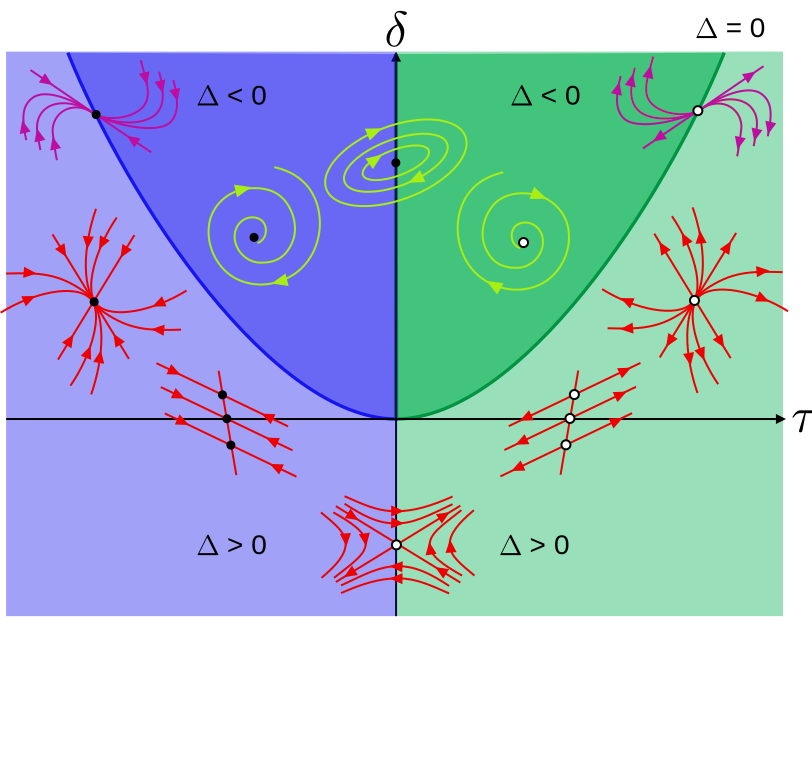
\includegraphics[width=3.8in]
{phase-plane/Phase_plane_nodes.png}
\caption{
$(\tau, \delta)$ plane
for $\dot{\vec{x}} = A \vec{x}$, where $A\in  \RR^{2\times 2}$ and  $\tau=\tr(A)$, $\delta=\det{A}$. This
figure  comes from Ref.\cite{wiki-phase-plane}}.
\label{fig-wiki-pp}
\end{figure}

First note that there is a unique fixed point iff 
$\det(A)=\delta\neq 0$.

\begin{itemize}
\item $\Delta < 0$
complex eigenvalues,
oscillations (perhaps damped)
\begin{itemize}[\checkmark]
\item $\tau>0$, exponential growth, spiral out
\item $\tau=0$, {\bf limit cycle}
\item $\tau<0$, exponential decay, spiral in
\end{itemize}


\item $\Delta = 0$
real eigenvalues,
no oscillations. $\tau^2 = 4\delta$
\begin{itemize}[\checkmark]
\item $\tau>0$, exponential growth, source
\item $\tau=0$, $\lam=0$, $\vec{x}$ is constant in time.
\item $\tau<0$, exponential decay, sink
\end{itemize}

\item $\Delta > 0$
real eigenvalues,
no oscillations 

\begin{itemize}[\checkmark]
\item both eigenvalues are negative, sink
\item both eigenvalues are positive, source
\item one eigenvalues ($\lam_-$) is negative 
and the other ($\lam_+$) is positive, saddle point. This 
includes case where $\tau=0$ so $\lam =\pm\frac{1}{2}\sqrt{\Delta}$.
\end{itemize}
\end{itemize}

